\documentclass[fleqn]{MJDArticle}
\usepackage{lscape}
\usepackage[colorinlistoftodos,prependcaption,textsize=tiny]{todonotes}
\usepackage{tablefootnote}
\bluelinks

\usepackage{cprotect}

\definecolor{umassblue}{RGB}{51,51,153}
\definecolor{blue}{RGB}{51,51,153}
\definecolor{red}{RGB}{153,0,51}

\newcommand\verbblue[1]{\textcolor[RGB]{51,51,153}{\textbf{#1}}}
\newcommand\verbred[1]{\textcolor[RGB]{153,0,51}{\textbf{#1}}}
\newcommand\verbgreen[1]{\textcolor[RGB]{0,51,51}{\textbf{#1}}}

\definecolor{Grey}{rgb}{0.95,0.95,0.95}
\usepackage{tikz}
\usetikzlibrary{fit,positioning}

\hypersetup{urlcolor=blue,citecolor = blue}
\renewcommand{\arraystretch}{1.1}
%%%%%%%%%%%%%%%%%%%%%%%%%%%%%%%%%%%%%%%%%%%%%%%%%%%%%%%%%%%%%%%%%%%%%%%
\begin{document}
\titleMA[\texttt{REmail}: A Set of Tools For Email Pre-Processing]{Matthew Denny, Neha Shah, Hanna Wallach, and Bruce Desmarais}
\large

\noindent Email continues to displace more traditional forms of communication in organizations as an efficient form of communication in certain domains. Email has a number of advantages from an organizations standpoint -- it is archival, easy to send to large groups of people, allows for attachments, can be centrally catalogued and searched, and is now increasingly available on mobile devices. Scholars seeking to understand social processes in these organizations, and industry data scientists looking to improve organizational performance have shown increasing interest in leveraging the vast amounts of information contained in organizational email archives. Yet the richness of email data, and its often proprietary format, can make analysis of these data at a large scale particularly challenging. In this report we detail a set of software tools and best practices for extracting useable textual and relational information from these data to facilitate statistical analysis of the content and structure of organizational email data. 

 
\begin{center}
	\begin{figure}[H]
		\centering
		\caption{\label{fig:email processing flowchart} Flowchart Detailing Steps in Email Processing for Social Science Aoplications.}
		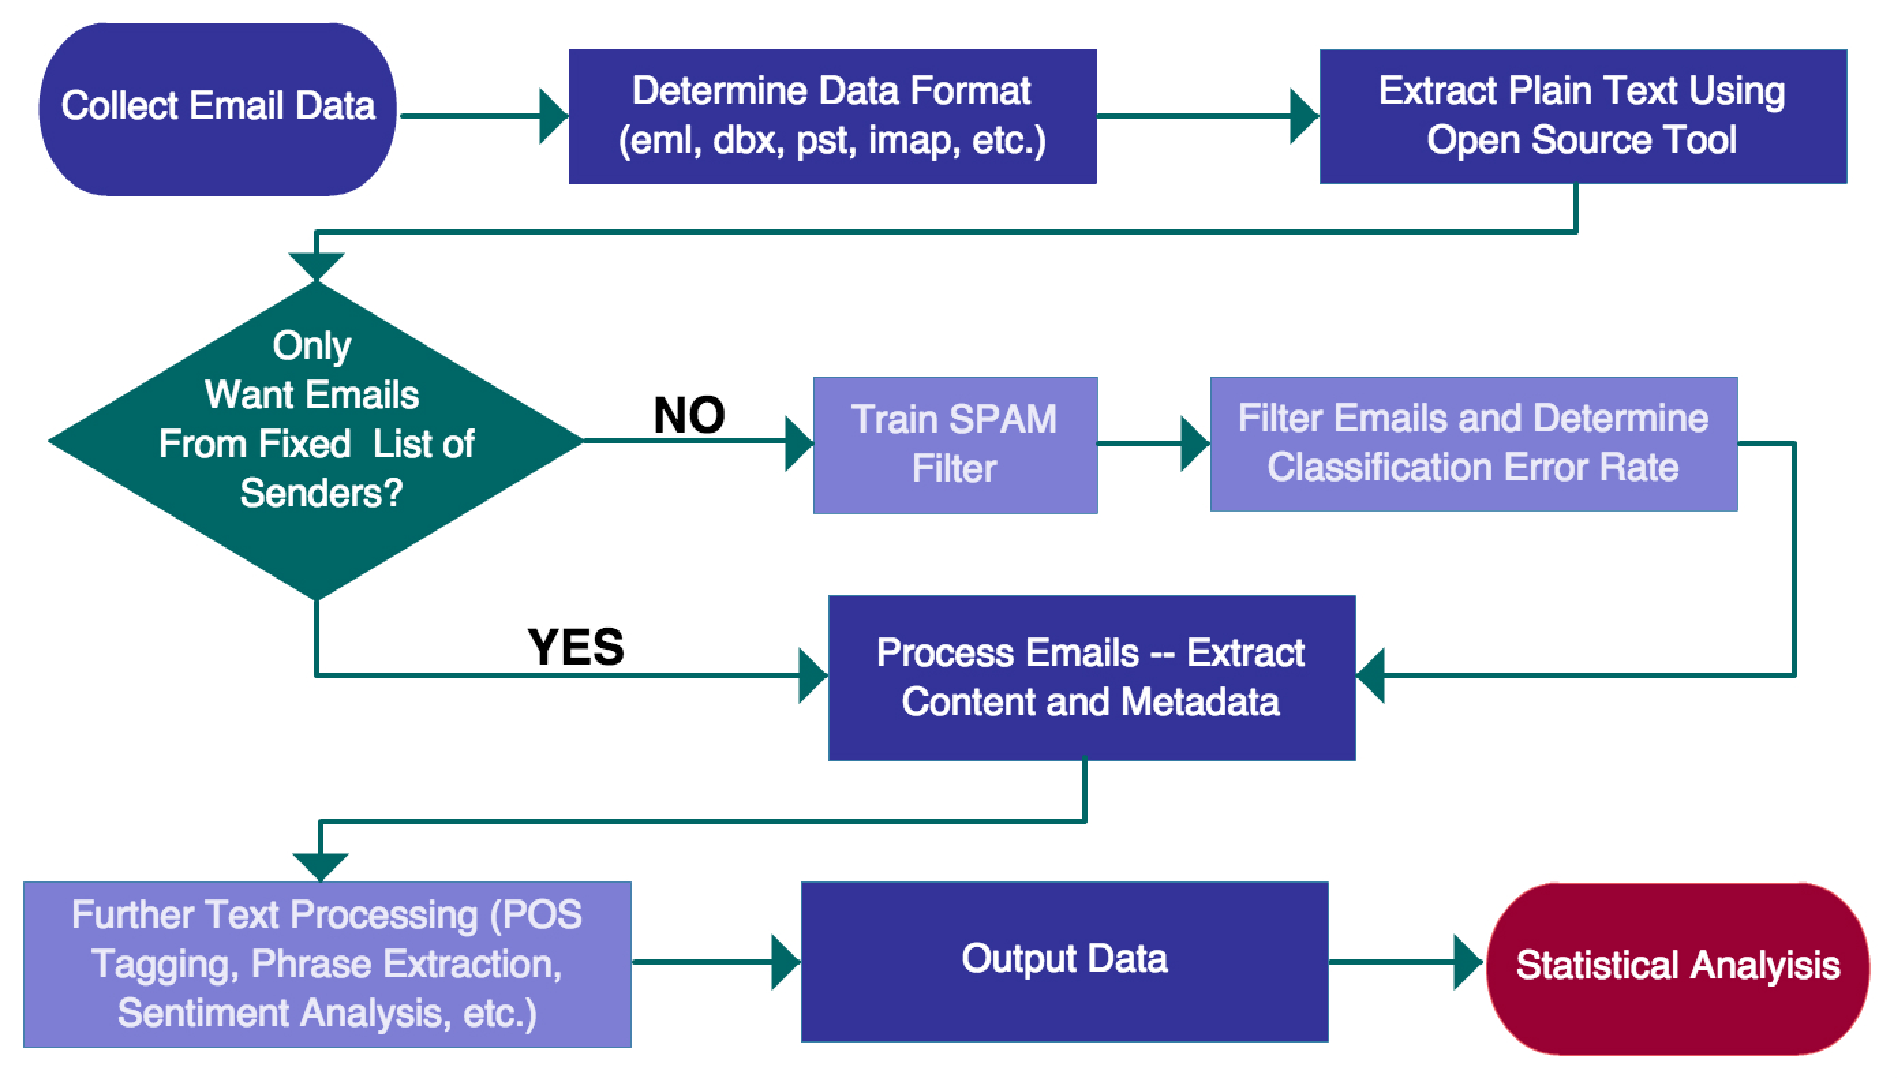
\includegraphics[width = .9\textwidth]{images/Email_Processing.pdf}
	\end{figure}
\end{center}

\noindent Figure \ref{fig:email processing flowchart} outlines the basic process explained in greater detail in the rest of this report. This approach was optimized and tested on a large cross-organizational corpus of approximately 500,000 emails and was found to provide high accuracy at relatively low time cost to the researchers. Throughout this report, we provide description and example code that was used to process the corpus described above, and use this example to illustrate best practices and potential pitfalls. At the end of this report, we introduce the \texttt{REmail} R package for semi-automated email processing and work through an example processing real email data. The user is expected to have mild competence using the command line and scripting in R, but our tools are designed to be user friendly and not overly time intensive.   

\section{Data Collection}

% \todo[inline]{ \large Describe the data we collected in 2103:\newline
%  -- What does it in clude, how many emails etc? \newline
%  -- Where from and why did we collect it?\newline
%  -- What it might be useful for.}

\noindent The tools described in this report were developed to process approximately 500,000 emails gathered in overlapping three-month periods in 2013 from seventeen North Carolina county governments. Each county provided three months of internal emails sent and received by department managers (Health, Finance, Utilites, etc.) in response to requests under North Carolina's public records disclosure laws. These data were collected as part of a field experiment testing for peer-effects in the compliance with public records requests (CITE Aaron et al.).  The raw volume of emails provided by each county ranged from about 2,000 emails to over 60,000\footnote{accommodations were made to prevent an undue burden being placed on the county governments.}. These counties represent both large and small population counties on both sides of the state with wide variation in median household income and racial composition. A map of county locations is provided in Figure \ref{fig:countyMap}. 

\begin{figure}[ht]
\centering
\caption{\label{fig:countyMap}North Carolina Counties Included in 2013 Data Collection Wave.}

\includegraphics[scale=1.5]{images/County_Map.pdf}
\end{figure}

\noindent We used the tools and approach described in the following sections to extract two (nested) datasets from this corpus -- all non-spam emails sent and received by the 362 department managers in our sample, and the subset of emails that were sent by a department manager and included atleast one other department manager in the ``To" or ``Cc" field. This resulted in reduced datasets of approximately 120,000 and 18,000 emails respectively, with a rich set of covariates for each manager and county, as well as text, and relational metadata for each email. (CITE OUR PAPER) introduces this dataset which will be made available for future studies. Email datasets such as the one described above provide a window into organizational dynamics, which may help researhers understand the institutional drivers of gendered patterns of communciation and performance more generally. 


\section{Raw Data: Format and Extraction to Plain Text}

\todo[inline]{ \large How to deal with raw email data:\newline
 -- What format did our data come in, what medium?, file sizes? \newline
 -- What tools did we use to extract the different kinds fo file. Provide lots of example code here and links to all of the project webpages. We want to really hold peoples hands here. \newline
 -- Talk about the output from these files and provide example plain text of a short email. Illustrate where the relevant information lies (I will do this with some cool verbatim highlighting).}
 
 Email data may be provided to the researcher in a number of different formats, some easier to deal with than others. When pssible, the researcher should request provision of data electronically in a common archival format such as the .pst or .dbx files that are relatively easily exported by Microsoft Outlook and Outlook Express respectively\footnote{Directions for bulk-exporting emails from Microsoft Outlook can be found at: \href{http://bit.ly/1PmNvIs}{http://bit.ly/1PmNvIs} and directions for exporting from Outlook Express can be found here: \href{http://bit.ly/1EaJaQD}{http://bit.ly/1EaJaQD}}, or in plain text or .eml format (with one file per email). Email data may also be provided in a number of other electronic formats depending on the particular client used but many of these formats are more challenging to convert to plain text (which is necessary for further processing). We discuss plain text extraction from some of these other formats in greater detail below, but applications such as MailStore\footnote{30 day free trial available at \href{http://www.mailstore.com/}{http://www.mailstore.com/}.} can also convert more obscure email data to a more standard format which can aide further processing. In general, the researcher should avoid acquiring email data in PDF\footnote{In certain cases, the \texttt{pdftotext} utility (\href{http://en.wikipedia.org/wiki/Pdftotext}{http://en.wikipedia.org/wiki/Pdftotext}) may provide acceptable character recognition performance, but it is the author's experience that email formatting may not be standardized, leading to additional challenges in automatic processing.} or paper form, as attempting to convert these documents to a useable digital format using optical character recognition is often extremely time intensive and may not provide very accurate results. \par
   County raw mail formats and statistics are presented in Table \ref{tab:county format}. .MAI,.imap,.txt and .eml are all txt formats, easy to parse with a property that there exists a file for each mail sent or received. The other two formats .pst and .mbox need to be converted to txt format. pst file formats are converted to txt files using the readpst utilities\footnote{Readpst utility to convert Outlook .pst files to other formats (\href{https://launchpad.net/ubuntu/precise/+package/readpst}{https://launchpad.net/ubuntu/precise/+package/readpst}) } \footnote{Man Page of readpst: \href{http://manpages.ubuntu.com/manpages/raring/man1/readpst.1.html}{http://manpages.ubuntu.com/manpages/raring/man1/readpst.1.html}}. Demo command line execution to convert a .pst file has been presented below. default.pst is the pst file which needs to be converted to text format. output\_directory is the directory where the extracted text file needs to be loaded.
\begin{code}
 readpst -So output_directory default.pst
\end{code}
 mbox is a Unix style mailbox. This Unix style mailbox is split into individual files using splitmbox code developed by Stuart Langridge \footnote{Stuart Langridge splitmbox.py: \href{http://www.kryogenix.org/code/}{http://www.kryogenix.org/code/} } \footnote{splitmbox.py code: \href{http://www.kryogenix.org/code/splitmbox.py.html}{http://www.kryogenix.org/code/splitmbox.py.html}}
 Demo command line execution is presented below. 
 \begin{code}
 python splitmbox.py default.mbox output_directory
 \end{code}
 default.mbox is the Unix style mailbox file which needs to be converted to txt. 
\begin{table}[ht]
\caption{\label{tab:county format} Raw file sizes and format for all county email corpora. The column  \textbf{Email Format} represents the raw format in which the email corpora was received. The column \textbf{Email Size} is the size of the corpora in its raw format. Column \textbf{Raw Email Count} provides total number of emails obtained after converting the corpora to text format.}
\centering
\begin{tabular}{lrrr}
  \hline
 \textbf{County} & \textbf{Email Format} & \textbf{Email Size} & \textbf{Raw Email Count} \\
  \hline
  \rowcolor{Grey}
Alexander & .pst &3.0GB & 26096 \\
Caldwell & .txt & 3.2GB & 21593\\
\rowcolor{Grey}
Chowan & .pst &9.0GB & 45192 \\
Columbus & .MAI &4.4GB &  31031 \\
\rowcolor{Grey}
Dare & .pst & 23.7GB & 68088 \\
Duplin & .imap & 6.9GB & 37330\\
\rowcolor{Grey}
Hoke & .eml & 3.4GB & 14874 \\
Jackson & .pst & 8.1GB & 72767 \\
\rowcolor{Grey}
Lenoir & .pst  & 4.3GB & 24343 \\
Lincoln & .pst  & 6.8GB  & 14075 \\
\rowcolor{Grey}
McDowell & .mbox & 0.96GB & 6184\\
Montgomery & .mbox & 1.9GB & 6527\\
\rowcolor{Grey}
Nash & .txt & 1.8GB & 10950 \\
Person & .pst & 3.8GB & 19616 \\
\rowcolor{Grey}
Transylvania & .txt & 4.7GB & 19639\\
Vance & .pst & 0.93GB& 5302 \\
\rowcolor{Grey}
Wilkes & .pst & 3.5GB & 18822 \\
   \hline
   \textbf{Totals:} &  & 90.3GB & 442429 \\
   \hline
\end{tabular}
\end{table}

\noindent Example text of an eamil originally recieved in \texttt{.pst} format after conversion to plain text using \texttt{libpst} is presented in Figure \ref{fig: example email plain text}. Some irrelevant metadata before and after the message was removed for clarity, but as we can see, the plain text contains a number of useful fields (that follow a common format across emails) such as the \textbf{Subject}, \textbf{Date}, \textbf{From}, \textbf{To}, and \textbf{Cc} (hightlighted in {\color{blue}blue}) and the email body text (hightlighted in {\color{red}red}). Importantly, emails extracted from \texttt{.pst} files also make use of a common message boundary delimiter:
\begin{verbatim}
--alt---boundary-LibPST-iamunique-
\end{verbatim}
\noindent which separates any quoted text from the body of the email and ensures that we do not capture an entire thread when processing an email (as we discard all text after encountering the second instance of this string at the start of a newline). The other email formats we processed posses similar message boundary strings, and we also look for the second instance of ``From" beginning a line as a backup method for avoiding including email threads when preprocessing emails.
  
\begin{center}
	\begin{figure}[ht]
		\centering
		\caption{\label{fig: example email plain text}Example plain text of an email extracted from a .pst archive using the \texttt{libpst} utility. Metadata is highlighted in {\color{blue}blue} and email body text is highlighted in {\color{red}red} for clarity. Note that emails archived in .pst format use a common delimiter between body and quoted text or attachments (illustrated on the last line of the example email). Email addresses have been redacted. }
\cprotect\fbox{ 
\begin{BVerbatim}[commandchars=\\\{\},frame=single]
...
\verbblue{Subject: NHC COPIERS}
\verbblue{Date: Tue, 22 Feb 2011 16:31:44 -0500}
X-MS-Has-Attach: yes
X-MS-TNEF-Correlator: 
Thread-Topic: NHC COPIERS
thread-index: AcvS1+Z0Errdm3IuQZWq9ZYmUiO7lg==
\verbblue{From: "Cain, Patty" <xxxxx@xxxxxx.xxx>}
\verbblue{To: "Seal, Donna" <xxxxx@xxxxxx.xxx>}
\verbblue{Cc: "Akin, Amy" <xxxxx@xxxxxx.xxx>, "Hight, Al" <xxxxxx@xxxxxx.xxx>}
MIME-Version: 1.0
Content-Type: multipart/mixed;
	boundary="--boundary-LibPST-iamunique-2004001971_-_-"
----boundary-LibPST-iamunique-2004001971_-_-
Content-Type: multipart/alternative;
	boundary="alt---boundary-LibPST-iamunique-2004001971_-_-"
--alt---boundary-LibPST-iamunique-2004001971_-_-
Content-Type: text/plain; charset="us-ascii"

\verbred{Donna,}
\verbred{I have added (and highlighted) Cooperative Extensions cost for copiers to}
\verbred{the NHC Inventory of Leased Copiers spreadsheet.  Not included in the}
\verbred{spreadsheet is XXX dollars (from 2009/2010) cost for print cartridges. }

\verbred{Also I just want to make you aware that in the period (2010) I figured}
\verbred{these numbers we were without 2 agent positions.  One of those has just}
\verbred{been hired and one is about to be hired.  With the addition of these two}
\verbred{people I would anticipate that our copy numbers will increase.}

\verbred{Patty}
...
--alt---boundary-LibPST-iamunique-2004001971_-_-	  
\end{BVerbatim}
}
	\end{figure}
\end{center}  

\section{Spam Email Filtering}
\todo[inline]{ \large Talk about how we filter spam emails out of our data:\newline
 -- Talk generally about the process at a high level and why it might be tricky. Show some example spam emails. \newline
 -- Talk about the different tools available and how we selected the tools we used. Any performance comparisons could go here -- or just links to thos project webpages.\newline
 -- Go mroe in depth into the tool we use, talk about how to use it and provide detailed example code.\newline
-- Talk about training classifier. \newline
-- Validation experiments -- how did we check to see how well we did, what are the error rates? Link to descriptive stats table in Output Format section where we will include a column on raw number of emails.\newline
 -- Discuss the limitations of spam filtering and what people need to watch out for.}

%now deal with external emails + spam filtering
While we are able to make use of bureaucratically compiled email addresses directly identify department managers, such metadata does not exist for the rest of the email addresses in our sample. Qualitative examination of the raw email data suggests that a large portion of the rest of emails in county manager inboxes are spam (sent from online marketers, retail chains, etc.). We make use of the Bogofilter\footnote{\href{http://bogofilter.sourceforge.net/}{http://bogofilter.sourceforge.net/}} filtering software to remove spam emails from the non manager-to-manager emails in our data. This filtering tool uses a variation on a naive Bayes classifier and requires that a sample emails be hand-coded as spam or not, in order to classify the rest of the emails in the corpus. We completed hand-training for each corpus using several thousand hand coded emails and post-hoc random checks of XXX classification decisions indicates that Bogofilter filter provides a very low false positive (9.1 percent) and  false negative rate (6.34 percent)\footnote{For a much more detailed explanation of the email filtering process see (CITE TECH REPORT), available (WEB-LINK).}. While the spam email classifier does not provide perfect results, our analyses of these emails only make use of listserv activity, which due to the nature of the filtering algorithm is very unlikely to be confounded by any classification errors. County email and manager statistics are presented in Table \ref{tab:county email summaries} and include the gender of county managers which are incorporated in our analysis of content-conditional assortative mixing between managers in these counties.  

\begin{center}
	\begin{figure}[ht]
		\centering
		\caption{\label{fig:spam1}Example of a Spam Mail in A Manager's Inbox  }
\cprotect\fbox{ 
\begin{BVerbatim}[commandchars=\\\{\},frame=single]
...
\verbblue{Date: Thu, 29 Mar 2012 23:45:37 -0700}
\verbblue{From: Kohl's <kohls@email.kohls.com>}
Reply-To: Kohl's <reply@email.kohls.com>
\verbblue{Subject: Save Up to 30\% On Everything + Free Shipping, No Minimum}
List-Unsubscribe: <mailto:unsubscribe-kohls.46036@interactexpress.net>
X-sgxh1: tOopkgHglxJhQHtLzfHgKLjQgJQmk
X-rext: 4.interact2.EhwpjicBmMXLTCwAhvLbQJrio9N1BJf8
X-cid: kohls.46036.11922
\verbblue{To: <lwhisnant@co.alexander.nc.us>}

--alt---boundary-LibPST-iamunique-14610823_-_-
Content-Type: text/plain; charset="utf-8"

\verbred{Shop the Big Weekend Sale featuring Extra Extra Specials.}
\verbred{<http://email.kohls.com/pub/cc?_ri_=X0Gzc2X\%3DWQpglLjHJlTQGoOirpJ7ufzce28O6oNe}
\verbred{IzacjphDvS7cMCVXtpKX\%3DBYYART&_ei_=EudOGAIid8eTVaybGhicyEh30vNXtoSJHPQitS8tsdObi}
\verbred{Uzwtl1DP1DphUS9FsoCP4ozazLVFa7RMD_h82CCRty06FT5f29P1MhaJyb0.>  }
\verbred{| View this e-mail in a Web browser }
\verbred{<http://email.kohls.com/pub/sf/FormLink?_ri_=X0Gzc2X\%3DWQpglLjHJlTQGoOirpJ7ufzce2}
\verbred{8O6oNeIzacjphDvS7cMCVXMtX3DWQpglLjHJlTQGgTJ4ekSoOUEA5K5JIdzfzeuvj5UzavhKmj&_ei_=Eu}
\verbred{dOGAIid8eTVaybGhicyEir1D7eTZjVi4gUwEXFIL3PCIBYBfy3kH30nc92KGuLwxHLLg.>}

\verbred{FREE SHIPPING NO MINIMUM! Free standard shipping.}
\verbred{Promo Code FUN2BFREE Surcharges still apply.}

\verbred{Kohl's Charge offer is good on all sale-, regular- and clearance-priced merchandise.}
\verbred{Offer not valid for price adjustments on prior purchases, the purchase of Gift Cards,}
\verbred{payment on a Kohl's Charge account or in conjunction with any percent-off discounts, }
\verbred{including age-specific discounts. Offer also not valid on the purchase of Kohl's Cares}
\verbred{cause merchandise or other charitable items. Excludes sales tax and shipping.}
\verbred{Subject to credit approval.See store for details.
}
...
\end{BVerbatim}
}
	\end{figure}
\end{center}  


\begin{center}
	\begin{figure}[ht]
		\centering
		\caption{\label{fig:spam2}Example of a Spam Mail in A Manager's Inbox  }
\cprotect\fbox{ 
\begin{BVerbatim}[commandchars=\\\{\},frame=single]
...
\verbblue{Date: Fri, 21 Sep 2012 16:46:57 -0400}
\verbblue{From: Strohman Enterprise <joe@strohmanenterprise.com>}
Reply-To: <joe@strohmanenterprise.com>
\verbblue{To: <dwayne.goodwin@chowan.nc.gov>}
\verbblue{Subject: New product from Garmin!}
X-Mailer: Roving Constant Contact 2009 (http://www.constantcontact.com)

\verbred{Having trouble viewing this email? Click here <http://campaign.r20.constantcontact.com/rendera}
\verbred{llr=5gztkndab&v=001sR9KXnYiTHgRbWWtkNYXEc86TCjBHvHZWWnbn2QGtAwZhK2IAJtj8fqroMQzFM33itkOUglV5Rf}
\verbred{AfjvUWFxNKfPS8rwo83G1RJRlxH-LCBK0cMaaUAFn-G6fTzZ8UvlJ4yo97_ubORS51r13O_QCal-AUQPBlKsydLn1unuWp}
\verbred{4phFEeM2hCE9DPpcbEnYyEbavBinJmPE8_Hl5pDvAkGvqPdUUZ9E0wRLS2Oiq_dyT5GrhC57T1dCM3AR4Iq2k7kZRSelvL}
\verbred{Mr1ZX-6Miljdte6KVAYauoSG2NpCPY5OKYka2kBSGaE4gjc54N0MmiTVkQYGMHgmvwg%3D>}

\verbred{STROHMAN ENTERPRISE}
\verbred{ <http://img.constantcontact.com/letters/images/1101093164665/nature_header3.jpg>}

\verbred{fenix}

\verbred{Utilizing our leading GPS technology, fçnix provides comprehensive navigation and tracking }
\verbred{functionalities as well as trip information to guide you on and}
\verbred{<https://static.garmincdn.com/en/products/010-01040-00/g/cf-lg.jpg#>}
\verbred{off the beaten track. Its built-in sensors provide information on heading, elevation and}
\verbred{weather changes. It's built to endure the toughest outdoor conditions - and also makes a }
\verbred{stylish day-to-day timepiece.}

\verbred{Features:}
\verbred{*       Altimeter}
\verbred{*       Barometer}
\verbred{*       Compass}
\verbred{*       Temperature}
\verbred{*       Wireless Communication}

...
\end{BVerbatim}
}
	\end{figure}
\end{center}  

Two types of spam filtering algorithms have been widely explored in literature, rule based classifiers and bayesian classifiers. Rule based classifiers have a set of rules and if a mail satisfies the rules with a certain score then the mail is classified as spam. Figure \ref{fig:spam2} and Figure \ref{fig:spam1} show two example spam emails.  Filtering out such emails becomes easy by just considering the presence of words like "trouble viewing this email", "discount" etc. Initially such rules work and help to segregate a large section of spam and ham emails. But as the rules become stricter recognizing the last few percent of spam email becomes difficult. Furthermore, rules need to be updated manually as  more spam is received. In contrast, bayesian classifiers use bag of words features to identify spam email and can be implemented in continuous learning mode with no manual intervention other than labeling the incoming mail as spam and non-spam. The most widely used bayesian filtering algorithm is Paul Graham algorithm\footnote{Paul Graham Algorithm: \href{http://www.paulgraham.com/spam.html}{http://www.paulgraham.com/spam.html}}

\begin{table}[ht]
\caption{\label{tab:packages} Few softwares available for spam classification.}
\centering
\begin{tabular}{p{5cm}p{12cm}}
  \hline
 \textbf{Package/Software} & \textbf{Comments} \\
  \hline
  Bogofilter\tablefootnote{Bogofilter page: \href{http://bogofilter.sourceforge.net/}{http://bogofilter.sourceforge.net/}} & Implements Paul Graham algorithm with changes suggested by Gary Robinson in 'A Statistical Approach to Spam Problem' \tablefootnote{Changes suggested by Gary Robinson \href{http://www.linuxjournal.com/article/6467}{http://www.linuxjournal.com/article/6467}} \\
  Spambayes\tablefootnote{Spambayes page: \href{http://spambayes.sourceforge.net/}{http://spambayes.sourceforge.net/}} & Spambayes also implements the Paul Graham algorithm with few modifications of its own.\\
  Spamprobe \tablefootnote{Spamprobe page: \href{http://spamprobe.sourceforge.net/}{http://spamprobe.sourceforge.net/}} & Spamprobe borrows its basic ideas from Paul Graham algorithm but is not the actual implementation of the algorithm. This package implements some tweaks in a way to improve effectiveness of the classifier. \\
  CRM114 Discriminator\tablefootnote{CRM114 Discriminator page: \href{http://crm114.sourceforge.net/}{http://crm114.sourceforge.net/}} & CRM is a system to filter incoming files, using various criterion. Criterion of categorization can be regexes, Hidden Markov models etc.\\
 \hline
\end{tabular}
\end{table}
%\footnotetext{Bogofilter page: \href{http://bogofilter.sourceforge.net/}{http://bogofilter.sourceforge.net/}}
%\footnotetext{Changes suggested by Gary Robinson \href{http://www.linuxjournal.com/article/6467}{http://www.linuxjournal.com/article/6467}}
%\footnotetext{Spambayes page: \href{http://spambayes.sourceforge.net/}{http://spambayes.sourceforge.net/}}
%\footnotetext{Spamprobe page: \href{http://spamprobe.sourceforge.net/}{http://spamprobe.sourceforge.net/}}
%\footnotetext{CRM114 Discriminator page: \href{http://crm114.sourceforge.net/}{http://crm114.sourceforge.net/}}

We use bogofilter for spam classification. Not only does it implement Paul Graham algorithm with some variation. But also provides a nice command line interface for training and classification. Bogofilter classifies email as spam, ham and unsure. Most of the unsure emails are ambigious mails which need a little manual intervention to be classified as spam or ham. After bogofilter classification, we classify all unsure mails sent by county officials and have been forwarded or replied to in the ham(non-spam) category.

\subsection{Training}
Paul Graham based Naive Baiyes Spam classification algorithm requires to be trained before it can be used to classify mails. We manually classify 9953 emails from the Nash County dataset. Training split consists of 7075 non spam emails and 546 spam emails. Command line interface for bogofilter is available.\footnote{Bogofilter man page: \href{http://linux.die.net/man/1/bogofilter}{http://linux.die.net/man/1/bogofilter}}. Bogofilter command line arguments for training spam emails is as follows:
\begin{code}
bogofilter -s -v < spam_filename
\end{code}
Bogofilter command line arguments for training ham emails is as follows:
\begin{code}
bogofilter -n -v < ham_filename
\end{code}
We have written a script training.py to train an entire directory as ham or spam. For training all ham emails, the emails are moved to a single directory and the directory name is given as command line argument to training.py. The code loops through individual files and trains the bogofilter classifier.
\begin{code}
python training.py ham ham_directory_name
\end{code}
For training an entire directory of spam emails the command line arguments are as follows:
\begin{code}
python training.py spam spam_directory_name
\end{code}
After training bogofilter a word directory gets created in the default bogofilter working directory. The training can be replicated across machines by sharing this wordlist.db. 
% Code for training
\subsection{Validation}
The validation split from the manually classified data consists of 1790 non spam emails and 142 spam emails.
On testing the classifier on validation split, a false postive rate of 9.1\% and false negative rate of 6.34\%. 
Command line arguments to classify a given mails as spam , ham or unsure is as follows:
\begin{code}
bogofilter -p -e < filename.txt > classified.txt
\end{code}
In this code, filename.txt represents the email which needs to be classified, and classified.txt contains one more header attribute called X-Bogosity which indicates whether the email is spam or not.
To loop through all the files in a folder and classify them as spam, unsure and ham and also filter unsure emails as spam and ham (all unsure emails which are forwards or replies or sent from county's domain names are classified as ham), we have written a script which can be executed as follows:
\begin{code}
python all_code_classification.py COUNTY_NAME input_directory output_directory
\end{code}
After running this code, the output\_directory will contains three folders ham,spam and unsure classified accordingly.
\subsection{Limitations}
This one classifier trained on Nash County emails is then used to classify emails from all other counties. Even though the nature of emails is same, their contextually they may vary. Hence, training on a different county and classifying on different county may not always be useful. For this reason, 20 random classified emails from each spam and ham are manually checked. If more than one email is found to be misclassified, then the classifier is discarded for that county. A different classifier needs to be trained for such exceptions.  For counties like Caldwell, where the email length is considerably smaller than Nash county, it is found that this classifier doesn't work.

\section{Email Processing}

\todo[inline]{ \large Walk through processing raw email data into usefable format:\newline
 -- General overview (MATT will do this) \newline
 -- Discuss why we are using python, what packages we are relying on and other alternatives to what we are doing. \newline
 -- Talk about the pipeline: (finding email addresses if we jsut want a subset of senders), extracting addresses, to, from ,cc, subject, body, time, removing quoted text, any challenges with each of these. \newline
 -- Speed, scalability and robsutness.\newline
 -- validation experiments in detail.\newline}
 
%discuss stopword removal, document representation, metadata coding (female names) and ethics of releasing data.
After identifying the subsets of manager-to-manager and non-spam manager-non-manager emails, the data were then fed through a preprocessing pipeline to represent the data in a form more amenable to statistical analysis\footnote{Python and R code to preprocess these emails is available at LINK TO GIT REPO.}. Each email had special characters, numbers and generic stopwords (i.e., function words, such as ``the,'' ``and,'' ``to,'' ``is,'' and ``that''), as well as some domain-specific stopwords removed. This is a common practice in the statistical topic modeling literature \citep{Wallach2009} and tends to increase the interpretability of output from these models as stopwords tend to be very high frequency, and may obscure topical content\footnote{A complete list of all stopwords removed during preprocessing is available LINK.}. Each email was then represented as a document-term vector (with one entry for each unique term in the vocabulary and the count of that term in the document), and a document-edge vector (with one entry for each possible recipient and a 1 in an entry indicating that person was a recipient of the current email). This form of data representation does disregard word ordering, but the ``bag-of-words" representation has been shown to yield high quality analyses and is very common in the statistical text analysis literature \citep{Grimmer2013}. Metadata, including: name, email, department, and gender was then coded for each manager in each county. Where possible, pictures of employees, voter registration records, or highly-gendered first names were used to assign a gender coding to each department manager\footnote{We recognize that gender may not be the most appropriate metric, and that our approach may miss those who self-identify as a different gender than their name may indicated, but we feel this choice of measurement is justified for privacy and practical reasons.}.


While the raw email data sets provided by these counties varied in size between 2,000 and 60,000 emails, a smaller portion of these emails are non-spam emails, with an even smaller subset of those non-spam emails actually being sent between managers. For our analyses of manager-to-manager communication patterns, we identified a set of email addresses for managers in each county using a published 2013 North Carolina county department manager directory, and implemented a set of software filtering tools to extract a subset of those emails sent by an manager that include at least one other manager in either the ``To:'' or ``Cc:" field. We do not perform any spam filtering on the emails sent between department managers as their email addresses positively identify these emails as non-spam. In our analyses we consider patterns of email communication indicated by ``To:'' and ``Cc:" fields both separately and combined, as the communication implied by ``Cc"ing a recipient can be quite different than the communication implied by including that recipient in the  ``To:'' field. For example, the county manager (responsible for overseeing all departments) may be Cc'd on many emails that they are not expected to reply to, where as an email sent from the finance department manager ``To" the parks department manager may be more likely to warrant a reply. 
\par
% Complete the python email package thing.
We use the python package called email \footnote{Python email package: \href{https://docs.python.org/2/library/email.html}{https://docs.python.org/2/library/email.html}} for obtaining certain fields from the email. The code has been designed such that, it loops through all the emails one after the other. For each email, the "From" field is extracted. If a valid email id is not found in this field or a valid email id cannot be constructed from this field, then the email is skipped.  Similarly, "To" and "CC" fields are extracted. If no valid recipients are found, or no valid recipient emailid can be constructed from these fields then the email is skipped. Next, the date of the email is extracted. The dates maybe in different timezones format they are all converted to standard EST format. Next, the subject field is parsed. Preprocessing on the subject text provides a list of tokens. Preprocessing involves stopword removal, conversion to lowercase and removing special characters. Parsing the Body part of email is a bit tricky. It involves removing header, tail and various other meta data associated with the email. Body text is also tokenized after preprocessing. All these fields extracted are saved as a dictionary and appeneded to a list. Once, all the emails are parsed, the list of dictionaries is saved as a pickle file and the output matrices are created. The subsections below provided a detailed description of the entire process.

\subsection{Email Id Extraction}
The email package provides the "From","To" and "Cc" fields in text format. We need to extract email ids from this text. These email ids are structured in a variety of ways. Figure \ref{fig:email1} shows an example where the "To" field contained both Name and email address. Figure \ref{fig:email2} shows an example where only names of recipients are mentioned. But their email addresses have not been mentioned. In such cases, the email address is constructed from the name. Figure \ref{fig:email3} shows an example where recipients are just email addresses and do not contain any names. The same may apply to the "From" and "Cc" fields also.
% Insert image 1 here
\begin{center}
	\begin{figure}[ht]
		\centering
		\caption{\label{fig:email1} Example of an Email where name and email address both are present in the "To" field. The field has been highlighted in blue. The text of the field is extracted using the email package. And individual email addresses and names are obtained using regular expression.	}
\cprotect\fbox{ 
\begin{BVerbatim}[commandchars=\\\{\},frame=single]
...
Received: from NCWWDITMXMBX34.ad.ncmail ([169.254.8.151]) by
 NCWWDITMXCHB32.ad.ncmail ([::1]) with mapi id 14.02.0281.000; Fri, 3 Aug 2012
 15:14:59 -0400
From: "Stallings, Susanne" <susanne.stallings@chowan.nc.gov>
\verbblue{To: "Alons, Scott L" <scott.alons@chowan.nc.gov>, "Byrum, Carrie"}
\verbblue{        <carrie.byrum@chowan.nc.gov>, "Colombo, Holly" <holly.colombo@chowan.nc.gov>,}
\verbblue{        Connie Parker <csc930@mchsi.com>, Denise Bunch <denise_bunch@ncsu.edu>, Ginny}
\verbblue{ White <ccac@inteliport.com> }
Subject: Agenda
Thread-Topic: Agenda
Thread-Index: Ac1xq8RpX5m7Ii/hSBiac5HE/BGAYg==
Date: Fri, 3 Aug 2012 15:14:59 -0400
...
\end{BVerbatim}
}
	\end{figure}
\end{center}  
% Insert image 2 here
\begin{center}
	\begin{figure}[ht]
		\centering
		\caption{\label{fig:email2} Example of an Email where only the name is present in the "To" field. The field has been highlighted in blue. The text of the field is extracted using the email package. And individual email addresses and names are obtained using regular expression.	 }
\cprotect\fbox{ 
\begin{BVerbatim}[commandchars=\\\{\},frame=single]
...
From: "Greg Cronk" <gcronk@alexandercountync.gov>
Subject: EMCO Ping Monitor Professional 4.6.8: Ping statistics for 'Firewall (10.1.1.1)'
\verbblue{To: Cronk, Greg}
\verbblue{Cc: Koenig, Michael}
Date: Fri, 24 Feb 2012 14:31:21 +0000
MIME-Version: 1.0
Content-Type: multipart/mixed;
        boundary="--boundary-LibPST-iamunique-1220987661_-_-"
...
\end{BVerbatim}
}
	\end{figure}
\end{center}  
% Insert image 3 here.
\begin{center}
	\begin{figure}[ht]
		\centering
		\caption{\label{fig:email3} Example of an Email where only the email address is present in the "To" field. The field has been highlighted in blue. The text of the field is extracted using the email package. And individual email addresses and names are obtained using regular expression.}
\cprotect\fbox{ 
\begin{BVerbatim}[commandchars=\\\{\},frame=single]
...
Received: from exchmbx.darenc.govt ([::1]) by exchcashub.darenc.govt
 ([2002:d00b:a803::d00b:a803]) with mapi; Mon, 22 Oct 2012 11:48:29 -0400
From: <sandyf@darenc.com>
\verbblue{To: <kevind@darenc.com>, <kristyd@darenc.com>, <ereilly@darenc.com>}
Date: Mon, 22 Oct 2012 11:48:27 -0400
Subject: RE:
Thread-Index: Ac2wUqe177g7VsXKTROZF1LwgnvkCQAAEckwAAE8kMAABMQ2YAAAaOUg
Message-ID: <083FB8344F7EB44BBEC104F92C7B8E1B93D8A7DE7D@exchmbx.darenc.govt>
...
\end{BVerbatim}
}
	\end{figure}
\end{center}  
\par

\begin{center}
	\begin{figure}[ht]
		\centering
		\caption{\label{fig:results} List of name and email address pairs extracted from the "To" fields of  Figures \ref{fig:email1} ,\ref{fig:email2} and \ref{fig:email3} using Regular Expression. Further processing is done on these lists before the final of emails are obtained. Further processing involves constructing email address from name if email address is absent. And replacing with earlier used email address if the name was used before with a different email address.}
\cprotect\fbox{ 
\begin{BVerbatim}[commandchars=\\\{\},frame=single]
Email id and name pairs extracted from email of Figure \ref{fig:email1}
\verbblue{[('Alons, Scott L','scott.alons@chowan.nc.gov'),('Byrum, Carrie','carrie.byrum@chowan.nc.gov'),}
\verbblue{ ('Colombo, Holly','holly.colombo@chowan.nc.gov'),('Connie Parker','csc930@mchsi.com'),}
\verbblue{ ('Denise Bunch','denise_bunch@ncsu.edu'),('Ginny White','ccac@inteliport.com')]}

Email id and name pairs extracted from email of Figure \ref{fig:email2}
\verbblue{[('Greg Cronk','')]}

Email id and name pairs extracted from email of Figure \ref{fig:email3}
\verbblue{[('','kevind@darenc.com'),('','kristyd@darenc.com'),('','ereilly@darenc.com')]}
\end{BVerbatim}
}
	\end{figure}
\end{center}  
We handle all such cases by using regular expressions. A single regular expression is used to generate a list of name and email address pairs. If the name is not present it is generated as empty, and if email address is not present it is generated as empty. Figure \ref{fig:results} shows all pairs extracted from "To" fields of Figure \ref{fig:email1},  Figure \ref{fig:email2} and  Figure \ref{fig:email3} .
\par
If no email address is obtained in the name and email address pair, then the email address is generated from the name. Each county has its own standard way of constructing email address from the name. We implement a county specific logic to form the email address from the first name, last name, initial and county domain name. A single official may have multiple email addresses. A mapping of name to email address is maintained. Every name extracted by regular expression is then compared with the mapping to see if it already existed. If it already existed then the previous email id it was used with is used. If it didn't exist then the current name and email address pair is added to the mapping. 

% Mention the function which does this. 
The function parse\_addresses of text\_parsing.py implements this functionality. It takes as input the text extracted from any of the "From", "To" and "Cc" fields. Ultimately this function returns a list of email addresses which is then saved into the dictionary for further processing. The code below shows an example on the usage of parse\_addresses function. 
\begin{code}
# Email "To" field extracted using email package. Output is obtained as a string.
# This then fed as input to parse_addresses.
email_to_field = "Cronk, Greg"
list_addresses = parse_addresses(email_to_field)
# Output will be ["gcronk@alexandercountync.gov"]
\end{code}
\subsection{Email Date Extraction}

The emails which appear in sender's Sent Mails will also appear in Receiver's Inbox. We don't want to parse the emails two times or multiple times in case the email was sent to multiple people. Hence, a way to remove duplicate emails has to be figured out. We use the meta data extracted from each email and compare it with already parsed emails. If they match, then the current email is declared duplicate. The meta data we compare is "From","To","Subject" and "Date". While implementing this logic, the code contains a snippet for creating and updating this meta data dictionary. We use a dictionary instead of a list to improve run time efficiency. The "From", "To" and "Subject" fields will remain the same in sender's Sent Items and receiver's Inbox. But however the date maybe in different formats due to different mail clients or different timezones.  Figure \ref{fig:date} shows various types of date formats which are usually observed and handled by the code. 

\begin{center}
	\begin{figure}[ht]
		\centering
		\caption{\label{fig:date} Different types of date formats observed in emails}
\cprotect\fbox{ 
\begin{BVerbatim}[commandchars=\\\{\},frame=single]
\verbred{Tue, 9 Oct 2012 16:10:43 +0000}

\verbred{Wed, 15 Aug 2012 07:38:51 -0700 (PDT)}

\verbred{31 Oct 2012 08:00:52 -0400}
\end{BVerbatim}
}
	\end{figure}
\end{center}  

Hence, all dates need to be converted to a single standard format. If the dates are in any of these formats, they are converted to UTC time format. The timezone information (+xxxx) or (-xxxx) is extracted and added or subtracted respectively from the actual date to obtain UTC time.  Any dates out of this format, are skipped as unable to convert. And this event is logged in the logger file created. Figure \ref{fig:date2} shows the dates in Figure \ref{fig:date}  converted to UTC format.

\begin{center}
	\begin{figure}[ht]
		\centering
		\caption{\label{fig:date2} Dates in Figure \ref{fig:date} converted to UTC time format. }
\cprotect\fbox{ 
\begin{BVerbatim}[commandchars=\\\{\},frame=single]
\verbred{09 Oct 2012 16:10:43}

\verbred{15 Aug 2012 00:38:51}

\verbred{31 Oct 2012 04:00:52}
\end{BVerbatim}
}
	\end{figure}
\end{center}  


\subsection{Email Subject Extraction}
The email subject can be extracted using the email python package as a string. But however the subject is not tokenized. Processing done to tokenize the subject involves these steps in the same order.
\begin{itemize}
\item 
\item All special characters and digits are removed from the text. Only alphabets (lower case or upper case are allowed to remain in the text.)
\item The text is converted to lower case.
\item Stopwords are removed from the list of tokens generated.
\end{itemize}
\begin{center}
	\begin{figure}[ht]
		\centering
		\caption{\label{fig:subject} Examples of subjects observed in emails. }
\cprotect\fbox{ 
\begin{BVerbatim}[commandchars=\\\{\},frame=single]
One valid subject

One more valid subject

One garbage subject
\end{BVerbatim}
}
	\end{figure}
\end{center}  


\subsection{Email Body Extraction}
\subsection{Code Output}
\subsection{Scalability and Time taken}


\subsection{Validation Experiments}

% Describe what gets missed in the validation experiments.
To ensure the accuracy of our automatic email processing techniques, a random sample of 20 emails included in the reduced data set was selected at random and audited manually to ensure that all authors, recipients and the content of the messages were recovered exactly. Results of these random manual audits indicate a 100\% accuracy rate across all counties, meaning that while we cannot rule out the possibility that emails were excluded from our data set due to the use of alternate (personal) email addresses, we are confident that we do not include emails that should not be in our manager-to-manager data set.

\subsection{Limitations}
The logic embedded for identifying same person with different email addresses, fails to work if no name is obtained with the email address. Since, the mapping exists only from name to email address. People with same name and different email address can be recognized. But, if the name is not obtained in the recipients then the logic fails. 
\par 
Email address construction from names has been hardcoded according to counties. To include any other format of email address construction, new code has to be written. A generic code does not exist for email address construction from county.


\section{Output Format}

\todo[inline]{ \large Describe how the output is formatted:\newline
 -- General overview (MATT will do this) \newline
 -- show lots of descriptive stats and talk abotu saving as Rdata files.}

Our email preprocessing tools generate intermediate output in \texttt{.csv} format, which is then packaged into a memory efficient and portable format and saved as an \texttt{.Rdata} file for further analysis or easy exporting to other formats through R. 

% %description of the data we are using for New Hannover, McDowell, Transylvania and Columbus counties
%
%
\begin{table}[ht]
\caption{\label{tab:county email summaries} Summary statistics for all county email corpora. The count of total emails are all non-spam emails we collected for a county including external and personal emails. The \textbf{Managers} column reports the total number of department managers in each county in our sample, while \textbf{Female} reports the number of those managers that were female at the time of data collection. The \textbf{Internal Emails} column records the total number of manager-to-manager emails in our dataset as identified by their official email addresses. Note that those lines which are left blank in the \textbf{Total Emails} and \textbf{Unique Recipients} columns pose addition challenges in automatic spam filtering so counts of non-spam emails are not available at this time.  }
\centering
\begin{tabular}{lrrrrr}
  \hline
 \textbf{County} & \textbf{Managers} & \textbf{Female} & \textbf{Internal Emails} &\textbf{Total Emails} & \textbf{Unique Recipients} \\
  \hline
  \rowcolor{Grey}
Alexander & 21 & 9 & 907 & 11924 & 10449 \\
Caldwell & 20 & 8 & 121 &  &  \\
\rowcolor{Grey}
Chowan & 23 & 11 & 2027 & 11737 & 7933 \\
Columbus & 24 & 10 & 920 & 12707 & 10895 \\
\rowcolor{Grey}
Dare & 27 & 12 & 2247 &  &  \\
Duplin & 27 & 14 & 1914 &  &  \\
\rowcolor{Grey}
Hoke & 24 & 11 & 1106 & 5565 & 1221 \\
Jackson & 24 & 6 & 1499 &  &  \\
\rowcolor{Grey}
Lenoir & 20 & 5 & 560 & 10499 & 10945 \\
Lincoln & 22 & 7 & 573 & 8727 & 5526 \\
\rowcolor{Grey}
McDowell & 17 & 5 & 326 & 3494 & 3191 \\
Montgomery & 18 & 10 & 680 & 2465 & 1681 \\
\rowcolor{Grey}
Nash & 19 & 8 & 1147 & 9133 & 7068 \\
Person & 21 & 9 & 1491 & 14023 & 7171 \\
\rowcolor{Grey}
Transylvania & 20 & 4 & 1857 & 14088 & 9479 \\
Vance & 18 & 8 & 185 & 4349 & 4387 \\
\rowcolor{Grey}
Wilkes & 17 & 2 & 303 & 8443 & 9693 \\
   \hline
   \textbf{Totals:} & 362 & 139 & 17863 & 117154 & 89639 \\
   \hline
\end{tabular}
\end{table}


\section{R Package Example}

\todo[inline]{ \large Talk about our plans for an R package, discuss the flow of reading in data and cleaning it.:\newline
 -- provide a worked example on a toy dataset}
 
 %%%%%%%%%%%%%%%%%%%%%%%%%%%%%%%%%%%%%%%%%%%%%%%%%%%%%%%%%%%%%
\hypersetup{linkcolor=black}
\bibliographystyle{MJD_plainnat}
\bibliography{library}
 
 

\end{document}
